\documentclass{article}

% Importing packages
\usepackage{amsmath, amsthm, amssymb, amsfonts}
\usepackage{thmtools}
\usepackage{graphicx}
\usepackage{setspace}
\usepackage{float}
\usepackage[colorlinks=true, linkcolor=Blue]{hyperref}
\usepackage[utf8]{inputenc}
\usepackage{framed}
\usepackage[dvipsnames]{xcolor}
\usepackage{tcolorbox}
\newtcolorbox{mymathbox}[1][]{colback=white, sharp corners, #1}


\title{Lecture 19}
\author{Mauro Patimo}


\begin{document}
\maketitle
Let's place a double at the origin in a free stream with velocity $U_\infty$. At $r=a$, $u_r=u_{\theta}=0$.\\
\begin{align*}
    u_r&=U_\infty\cos\theta\left(1-\frac{a^2}{r^2}\right)\\
    u_\theta&=-U_\infty\sin\theta\left(1+\frac{a^2}{r^2}\right)
\end{align*}
So we can trace a closed circle with a radius of $a$ around the doublet. The streamlines are shown in Fig. \ref{fig:Streamlines around a doublet.png}. \\
\begin{figure}
    \centering
    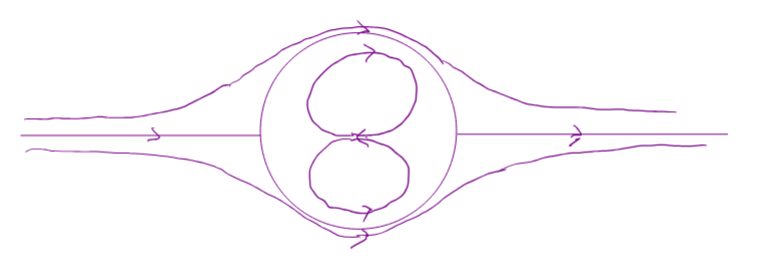
\includegraphics[width=0.8\textwidth]{Streamlines around a doublet.png}
    \caption{Streamlines around a doublet}
    \label{fig:Streamlines around a doublet.png}
\end{figure}
Since the circle represent a streamline, we can replace it with a solid body. The flow around the body will be the same as the flow around the doublet. This is a good way to represent a solid body in a flow.\\
We can notice how the the streamlines get closer to each other as the radius increases. Since our flow is incompressible, the velocity must increase as the radius increases. 
We can further explain this by thinking about conservation of mass. Since the area (or volume for a 3D case) decreases, and the density is constant, the mass has to find a way to be conserved. We can then think about the mass flux:
\begin{align*}
    m = \int_A \rho \vec{u}\cdot d\vec{A}
\end{align*}
Since we just said that the density is constant, and the area is decreasing, the velocity must increase. We can actually calculate the velocity at the surface of the body:
\begin{align*}
    u_\theta&=-U_\infty\sin\theta\left(1+\frac{a^2}{r^2}\right)_{r=a, \theta=\frac{\pi}{2} or \frac{3\pi}{2}}\\
    |u_\theta|&=2U_\infty
\end{align*}
We can also calculate the pressure coefficient, by comparing the pressure at a certain point ($P$), and the pressure of the flow at a point far away from the body ($P_\infty$), and the normalizing it with the dynamic pressure\footnote{The dynamic pressure is the pressure per unit volume of a fluid due to its velocity: $q=\frac{1}{2}\rho U_{\infty}^2$}:
\begin{align*}
    C_p&=\frac{P-P_\infty}{\frac{1}{2}\rho U_\infty^2}\\
    &=\frac{\frac{1}{2}\rho U_{\infty}^2 - \frac{1}{2}\rho V^2}{\frac{1}{2}\rho U_\infty^2}\\
    &=1-\left(\frac{V}{U_\infty}\right)^2
\end{align*}
The graph for the pressure coefficient is shown in Fig. \ref{fig:Pressure coefficient around a doublet}. The values on the axis are quite unusual. As they start from $1$ and end on $-3$ on the y-axis. The reason why a real flow doesn't match the theoretical curve is due to separation zones, that we'll look into in the future. As of right now, don't think about it.\\
Since the pressure coefficient will be the same and the opposite on the top and bottom of the body, the net force will be zero. This is called \textbf{D'Alembert's paradox}.\\
\begin{figure}
    \centering
    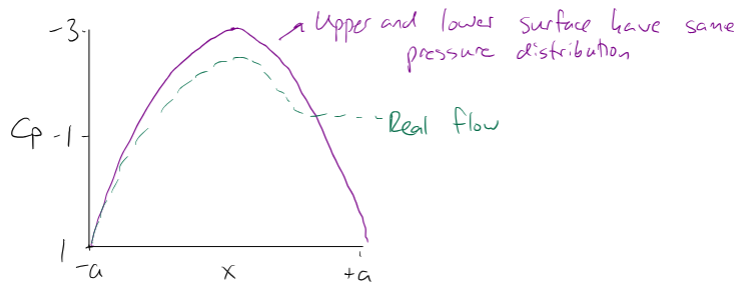
\includegraphics[width=0.8\textwidth]{Pressure coefficient around a doublet.png}
    \caption{Streamlines around a doublet}
    \label{fig:Pressure coefficient around a doublet.png}
\end{figure}
Since the cylinder surface is a perfect circle we can add a point vortex at the center of it and not change the surface shape, simplifying our calculations.\\
The velocity potential for a point vortex is:
\begin{align*}
    \phi_v=\frac{\Gamma}{2\pi}\ln r
\end{align*}
Add this to the velocity potential of the doublet:
\begin{align*}
    \phi=\underbrace{u_{\infty}(rcos\theta + \frac{cos\theta}{r}a^2)}_\text{Flow around circle}+\underbrace{\frac{\Gamma}{2\pi}\theta}_\text{Point vortex}
\end{align*}
The velocity field is now:
\begin{align*}
    u_r &= u_{\infty}\left(1-\frac{a^2}{r^2}\right)cos\theta\\
    u_\theta &= -u_{\infty}\left(1+\frac{a^2}{r^2}\right)sin\theta+\frac{\Gamma}{2\pi r}
\end{align*}
As you can see from the equations, the radial velocity is not influenced by the vortex, while the tangential velocity is.\\
The stagnation points are no longer at $\theta=0$ and $\pi$. In order to calculate them, we need to set $u_\theta=0$:
\begin{align*}
    0 &= -u_{\infty}\left(1+\frac{a^2}{a^2}\right)sin\theta+\frac{\Gamma}{2\pi r}\\
    sin\theta&=\frac{\Gamma}{4\pi u_\infty a}\\
\end{align*}
So in case $\Gamma=4\pi u_\infty a$, the stagnation point is at $\theta=\frac{\pi}{2}$.In case $\Gamma>4\pi u_\infty a$, the stagnation points will lift off the surface. As shown in Fig. \ref{fig:Stagnation point liftoff.png}. Remember that $\Gamma$ is measure in a counter-clockwise direction.\\
We can then find the force on the cylinder by integrating the pressure coefficient over the surface of the cylinder:
\begin{figure}
    \centering
    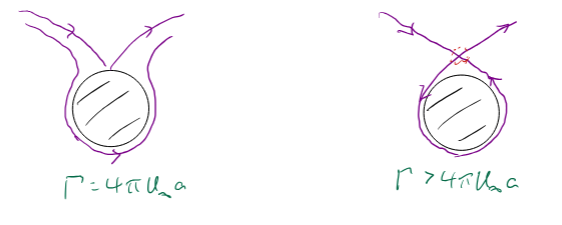
\includegraphics[width=0.8\textwidth]{Stagnation point liftoff.png}
    \caption{Stagnation point liftoff}
    \label{fig:Stagnation point liftoff.png}
\end{figure}
\begin{align*}
    F & = \int -P \hat{n} dA=\int -\frac{1}{2}\rho U_\infty ^2 \int C_p \hat{n} dA
    & = -\rho u_\infty \Gamma \hat{j}
\end{align*}
The force is perpendicular to the free stream velocity. This is called \textbf{Lift}. We can summarize the forces in the cylinder with two formulas:
\begin{mymathbox}
    \begin{align}
        L'&=-\rho u_\infty \Gamma \quad \text{(Kutta-Joukowsky Theorem)} \\
        D'&=0 \quad \text{(D'Alembert's Paradox)}
    \end{align}
\end{mymathbox}
\end{document}